\documentclass[]{scrartcl}

%%% PACKAGES
\usepackage[english]{babel}
%\usepackage[T1]{fontenc} % pouzije EC fonty
\usepackage[utf8]{inputenc} % set input encoding (not needed with XeLaTeX) 
\usepackage{lmodern}
\usepackage{graphicx} % support the \includegraphics command and options

\usepackage{caption}

\usepackage{subfig}
\usepackage{cite}

\usepackage{amsmath}

% poziti pro vypis kodu
\usepackage{listings}
\usepackage{xcolor}

\definecolor{mygreen}{rgb}{0,0.6,0}
\definecolor{mygray}{rgb}{0.5,0.5,0.5}
\definecolor{mymauve}{rgb}{0.58,0,0.82}
% sets appearance of listings
\lstset{ %
	backgroundcolor=\color{yellow!20},   % choose the background color; you must add \usepackage{color} or \usepackage{xcolor}
	basicstyle=\scriptsize,        % the size of the fonts that are used for the code
	breakatwhitespace=false,         % sets if automatic breaks should only happen at whitespace
	breaklines=true,                 % sets automatic line breaking
	captionpos=b,                    % sets the caption-position to bottom
	commentstyle=\color{mygreen},    % comment style
	deletekeywords={...},            % if you want to delete keywords from the given language
	escapeinside={\%*}{*)},          % if you want to add LaTeX within your code
	extendedchars=true,              % lets you use non-ASCII characters; for 8-bits encodings only, does not work with UTF-8
	frame=single,	                   % adds a frame around the code
	keepspaces=true,                 % keeps spaces in text, useful for keeping indentation of code (possibly needs columns=flexible)
	keywordstyle=\color{blue},       % keyword style
	language=C,                 % the language of the code
	otherkeywords={*,try, catch},           % if you want to add more keywords to the set
	numbers=left,                    % where to put the line-numbers; possible values are (none, left, right)
	numbersep=5pt,                   % how far the line-numbers are from the code
	numberstyle=\tiny\color{mygray}, % the style that is used for the line-numbers
	rulecolor=\color{black},         % if not set, the frame-color may be changed on line-breaks within not-black text (e.g. comments (green here))
	showspaces=false,                % show spaces everywhere adding particular underscores; it overrides 'showstringspaces'
	showstringspaces=false,          % underline spaces within strings only
	showtabs=false,                  % show tabs within strings adding particular underscores
	stepnumber=1,                    % the step between two line-numbers. If it's 1, each line will be numbered
	stringstyle=\color{mymauve},     % string literal style
	tabsize=2,	                   % sets default tabsize to 2 spaces
	title=\lstname                   % show the filename of files included with \lstinputlisting; also try caption instead of title
}

\title{RoVi1}
\subtitle{Final Project \vspace{2cm}}

\author{\textbf{Group:} Petr Batěk,  Bjarki Páll Sigurdsson, Salman Taj}


\begin{document}
	\selectlanguage{english}
	
	\maketitle
	
	\newpage

\begin{abstract}
\section*{Project Description}

\end{abstract}

\section{Tracking points using image Jacobian}
We have implemented algorithm for visual servoing in this part. For this part we selected specific marker points as described in problem statement and use mathematical camera model to get image pixel coordinates of the points. Image recognition thus wasn't used in this part.

To compute joint updates it was first needed to compose matrix $\boldsymbol{Z}_{image}$ as described in Robotics Notes:
\begin{align}
	\boldsymbol{Z}_{image}(\boldsymbol{q}) = \boldsymbol{J}_{image}\boldsymbol{S}(\boldsymbol{q})\boldsymbol{J}(\boldsymbol{q})\; 
\end{align}
where $\boldsymbol{J}(\boldsymbol{q})$ is manipulator Jacobian. For its computation we used function from RobWork library. $\boldsymbol{J}_{image}$ is image Jacobian matrix. We implemented function for its computation called \texttt{calculateImageJ} which can be found in the file \texttt{inverseKinematics.cpp}. We used fixed value for $z$ coordinate. Since we used frame \texttt{cameraSim} to model the camera we set $z\, = \, -0.5$ for every function call. Finally matrix $\boldsymbol{S}(\boldsymbol{q})$ was composed by inserting transpose of the rotational matrix $\boldsymbol{R}_{base}^{tool}$ twice to its diagonal.

The next information necessary to compute joints updates is difference or move of target points $\overrightarrow{\boldsymbol{dU}}_{image}$. We have programmed function \texttt{calculate\_dUImage} to solve for $\overrightarrow{\boldsymbol{dU}}_{image}$.

Having matrix $\boldsymbol{Z}_{image}$ and $\overrightarrow{\boldsymbol{dU}}_{image}$ it was possible to solve for joint positional update ${\boldsymbol{dq}}$ using method of Linear Least Squares.

We adapted two equations from robotics notes into single expression for ${\boldsymbol{dq}}$ computation:
\begin{align}
	\boldsymbol{dq} = \boldsymbol{Z}^T\left(\boldsymbol{Z}\boldsymbol{Z}^T\right)^{-1} \overrightarrow{\boldsymbol{dU}}_{image}
\end{align}
In this equation we used $\boldsymbol{Z}$ to denote $\boldsymbol{Z}_{image}$.
For this solving of this LSM problem we have implemented function \texttt{compute\_dQ\_LSM} which can be found in \texttt{inverseKinematics.cpp}.

\texttt{algorithm2} is the function, where are all of described functions organized together to compute joint updates $\boldsymbol{dq}$ base on the manipulator state and the error in image coordinates $\overrightarrow{\boldsymbol{dU}}_{image}$.

We have implemented $J_{image}$ and $\overrightarrow{\boldsymbol{dU}}_{image}$ composition in a scalable way, so the same functions can be used to track one or multiple target points.

Model of the robot manipulator has velocity limits on joint movements, so it was necessary to check if the limits were satisfied before joint updates. We did so by measuring time for update computations, subtracting this time from workcell update period specified by \texttt{deltaT} and finally we divided update $\boldsymbol{dq}$ by the result of subtraction. Velocity of joint movement is the result of the operation. By comparing the actual velocity with manipulator limits it was possible to find out if the limits are satisfied. If they aren't algorithm simply saturate joint movement in order to hold all conditions. For comparison and saturation, function \texttt{saturateDQ} was implemented.

In the following section we provide simulation results from tests of inverse kinematics.

\subsection{Simulation Tests}
During simulations, we recorded joint configurations, tool/camera frame position and orientation for $\texttt{deltaT} = 1000 ms$ and finally we performed tests for different values for \texttt{deltaT} in the range $50\, ms < \texttt{deltaT} < 1000\, ms$ and plotted maximum errors of 
$\overrightarrow{\boldsymbol{dU}}_{image}$

\subsubsection*{Slow Marker Sequence}
\begin{figure}[!htp]
	% Maximum length
	\subfloat[Tracking Single Point]
	{
		\label{fig:Slow1PointJoints}
		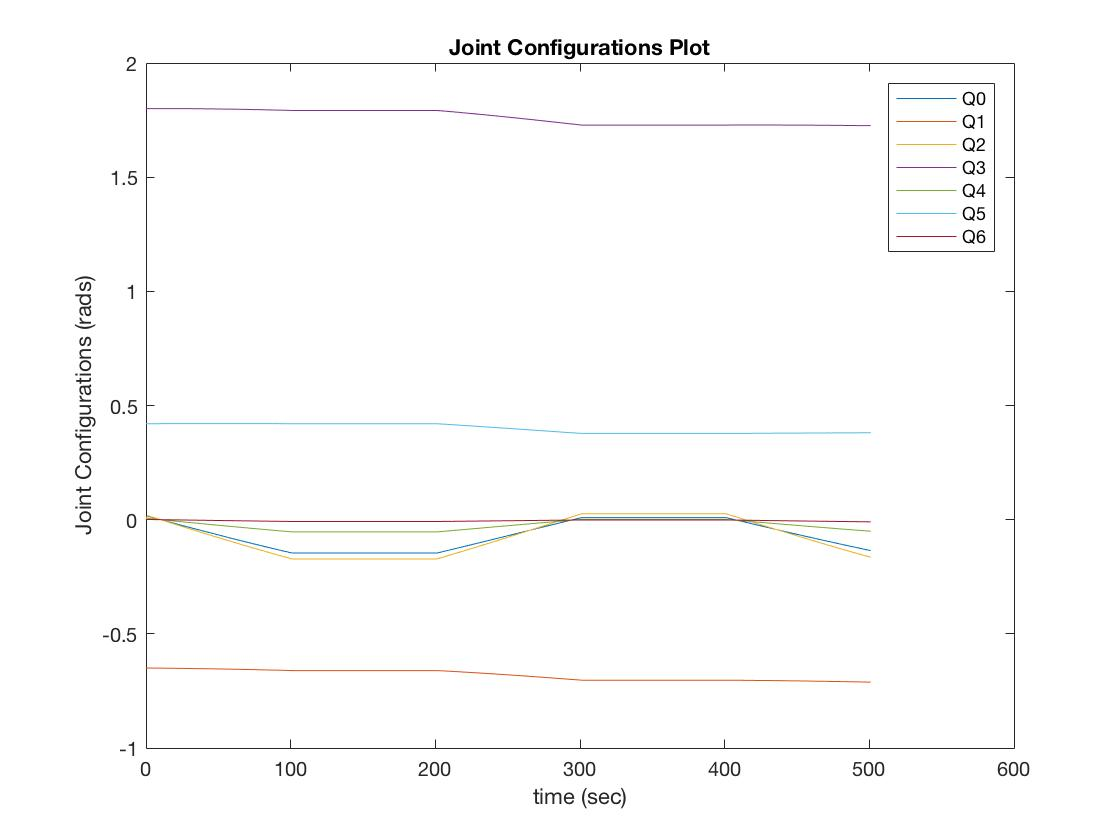
\includegraphics[width=0.49\linewidth]{fig/SlowSequence_joints_1_Targ_Pt.jpg}
	}\hfill
	\subfloat[Tracking 3 Points]
	{
		\label{fig:Slow3PointsJoints}
		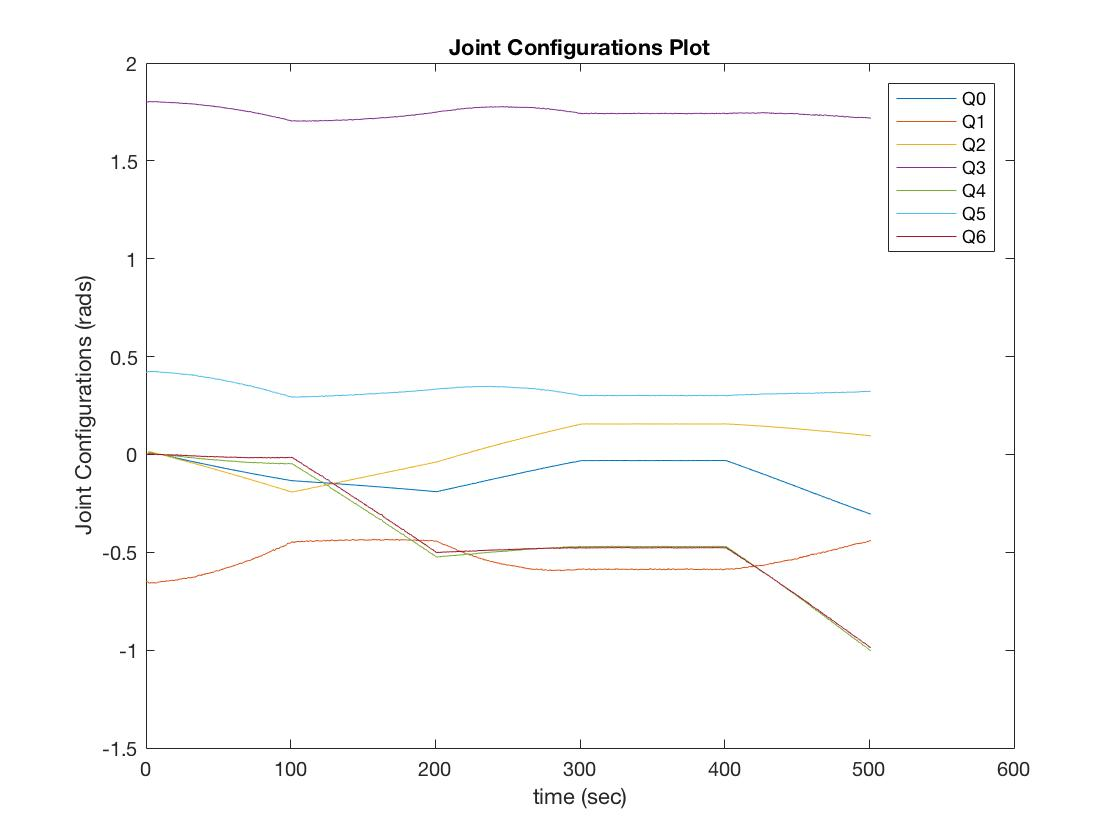
\includegraphics[width=0.49\linewidth]{fig/SlowSequence_joints_M_Targ_Pts.jpg}
	}%
	\caption{Joint configurations}
	\label{fig:SlowSequenceJoints}
\end{figure}

\begin{figure}[!htp]
	% Maximum length
	\subfloat[Tracking Single Point]
	{
		\label{fig:Slow1PointToolPose}
		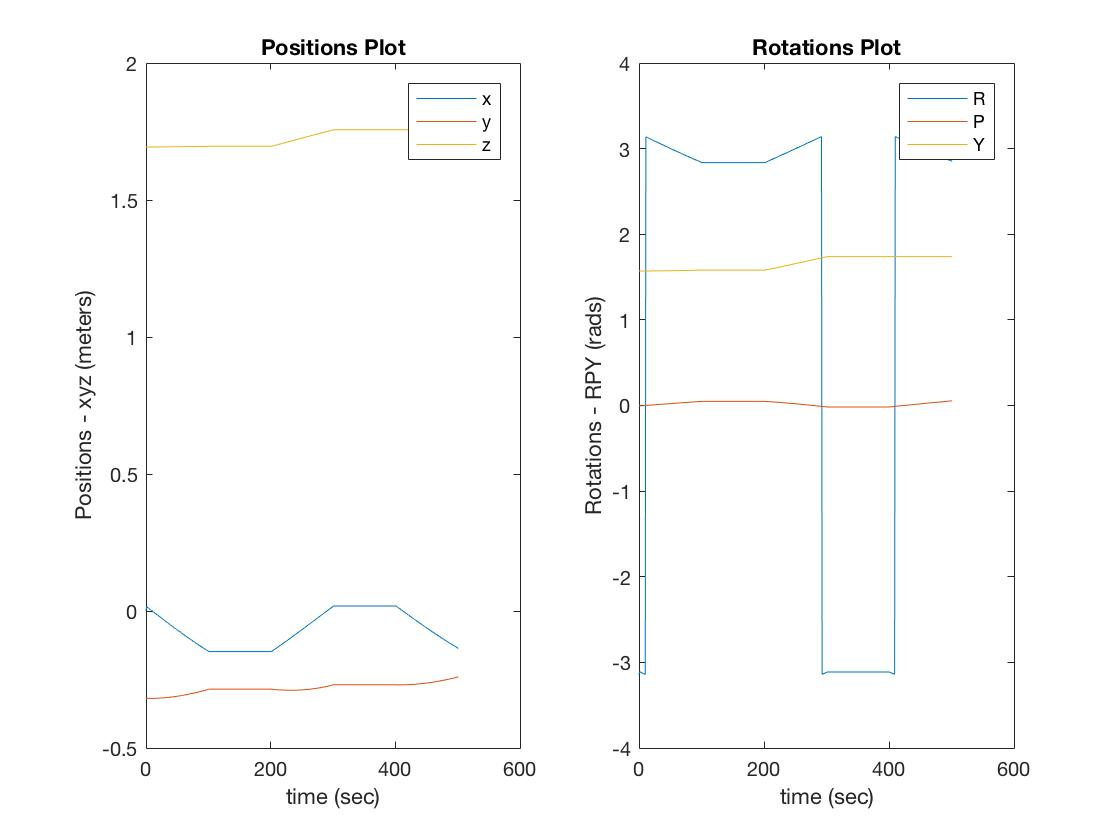
\includegraphics[width=0.49\linewidth]{fig/SlowSequence_tool_pose_1_Targ_Pt.jpg}
	}\hfill
	\subfloat[Tracking 3 Points]
	{
		\label{fig:Slow3PointsToolPose}
		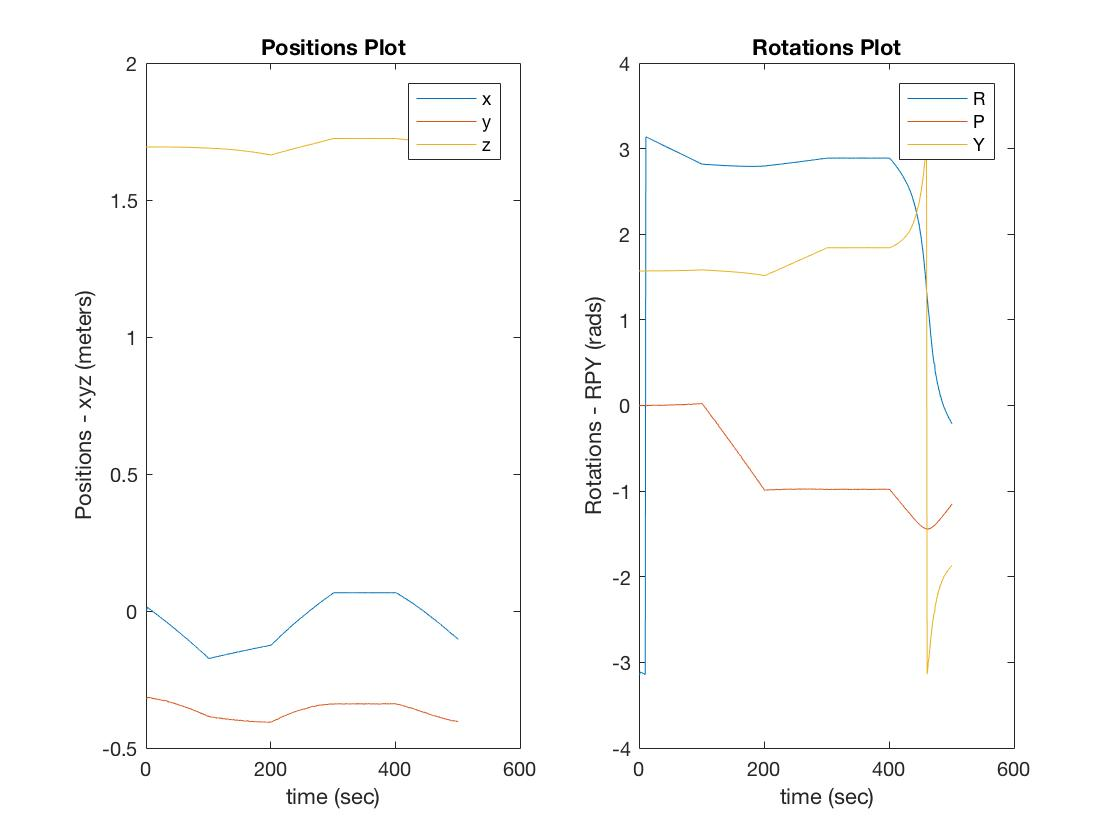
\includegraphics[width=0.49\linewidth]{fig/SlowSequence_tool_pose_M_Targ_Pts.jpg}
	}%
	\caption{Tool pose transformations}
	\label{fig:SlowSequenceToolPose}
\end{figure}
In figure \ref{fig:Slow1PointToolPose} and \ref{fig:Slow3PointsToolPose} are apparent jump in roll angle around $z$ axis. This however doesn't imply jumps in tool orientation. Abrupt jumps in the graphs were caused because of switching between $-\pi$ and $\pi$ rad angle. In the real world, change in orientation is small. Implementation of Robwork transformations probably keeps all orientation angles in the interval $ \langle -\pi, \; \pi \rangle $.

\subsubsection*{Medium Marker Sequence}
\begin{figure}[!htp]
	% Maximum length
	\subfloat[Tracking Single Point]
	{
		\label{fig:Medium1PointJoints}
		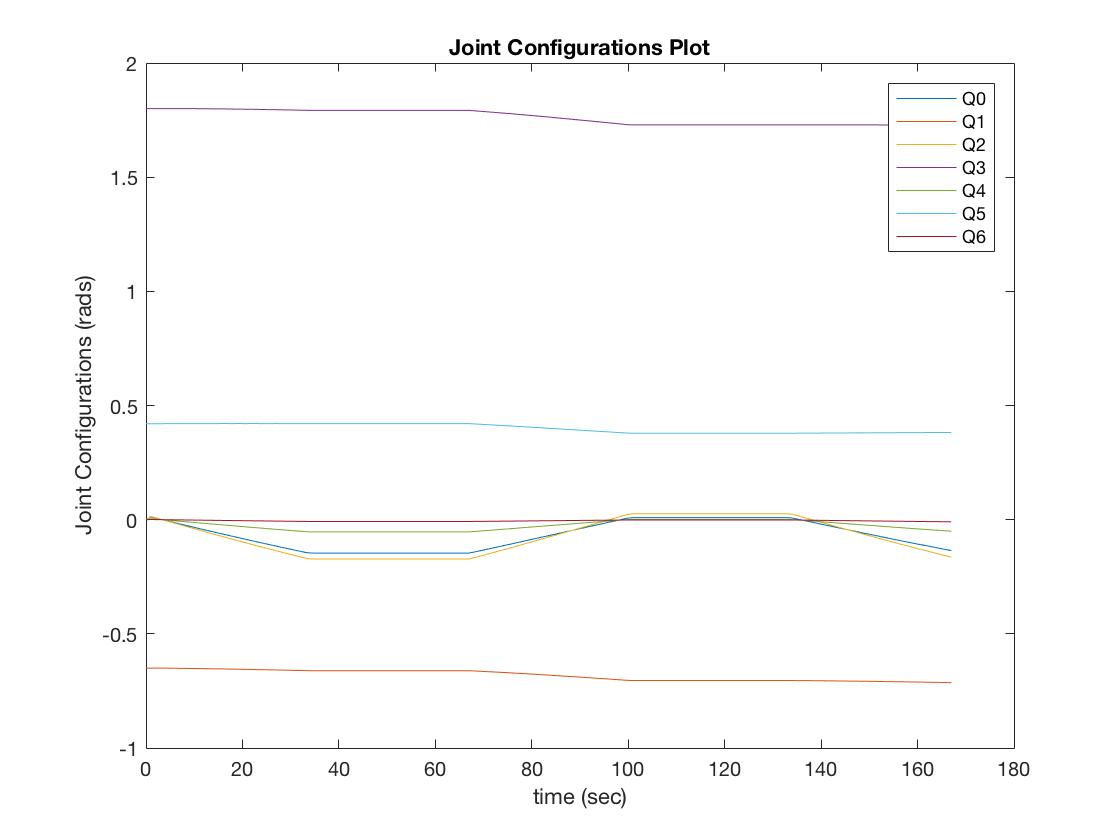
\includegraphics[width=0.49\linewidth]{fig/MediumSequence_joints_1_Targ_Pt.jpg}
	}\hfill
	\subfloat[Tracking 3 Points]
	{
		\label{fig:Medium3PointsJoints}
		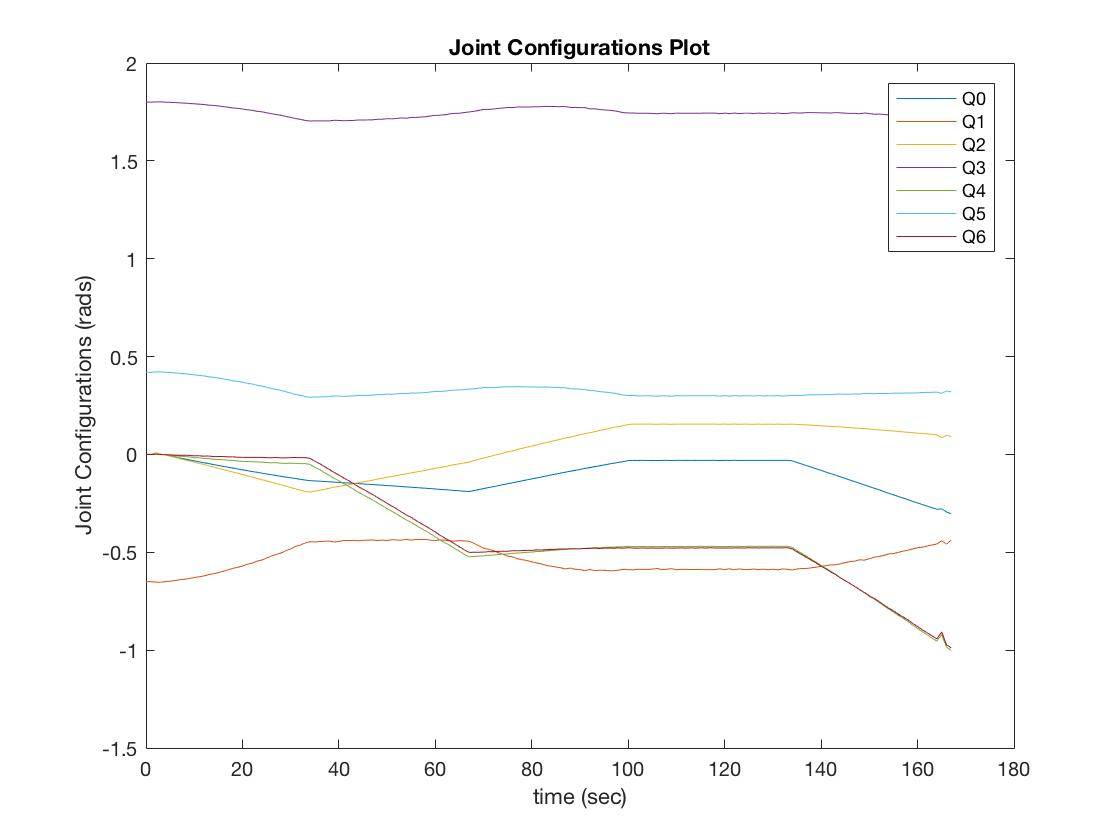
\includegraphics[width=0.49\linewidth]{fig/MediumSequence_joints_M_Targ_Pts.jpg}
	}%
	\caption{Joint configurations}
	\label{fig:MediumSequenceJoints}
\end{figure}

\begin{figure}[!htp]
	% Maximum length
	\subfloat[Tracking Single Point]
	{
		\label{fig:Medium1PointToolPose}
		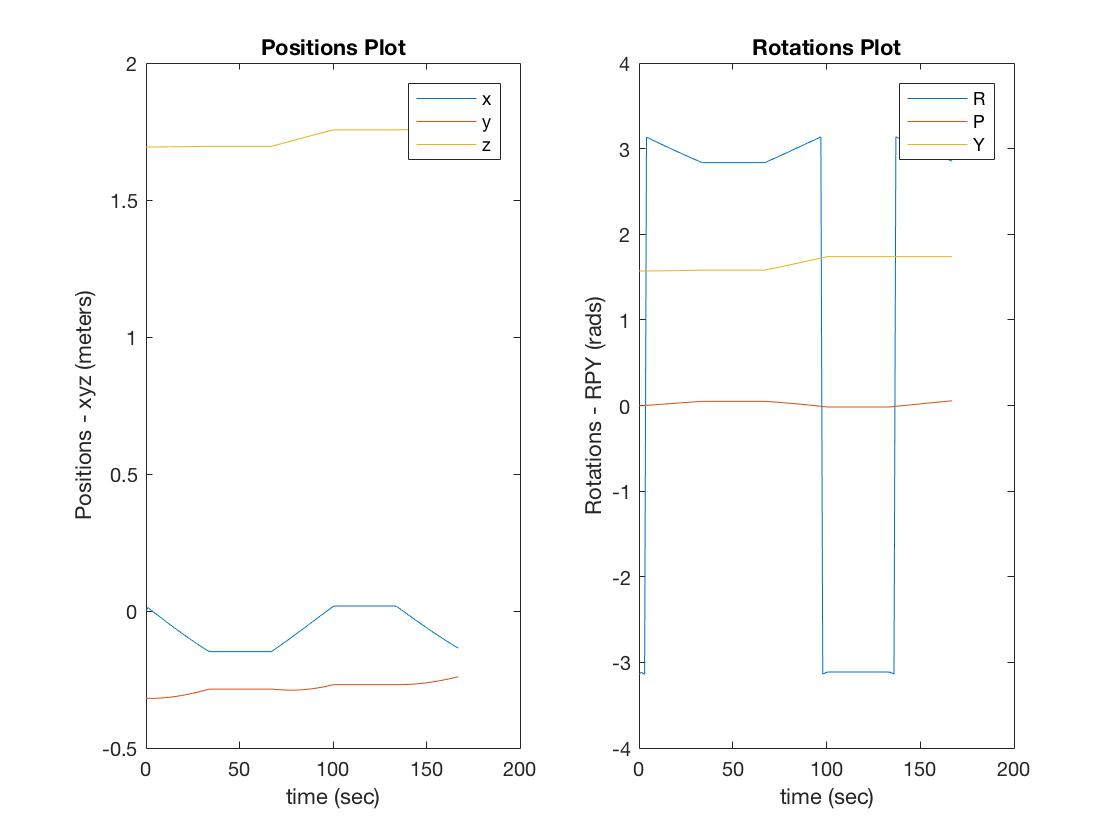
\includegraphics[width=0.49\linewidth]{fig/MediumSequence_tool_pose_1_Targ_Pt.jpg}
	}\hfill
	\subfloat[Tracking 3 Points]
	{
		\label{fig:MediumPointsToolPose}
		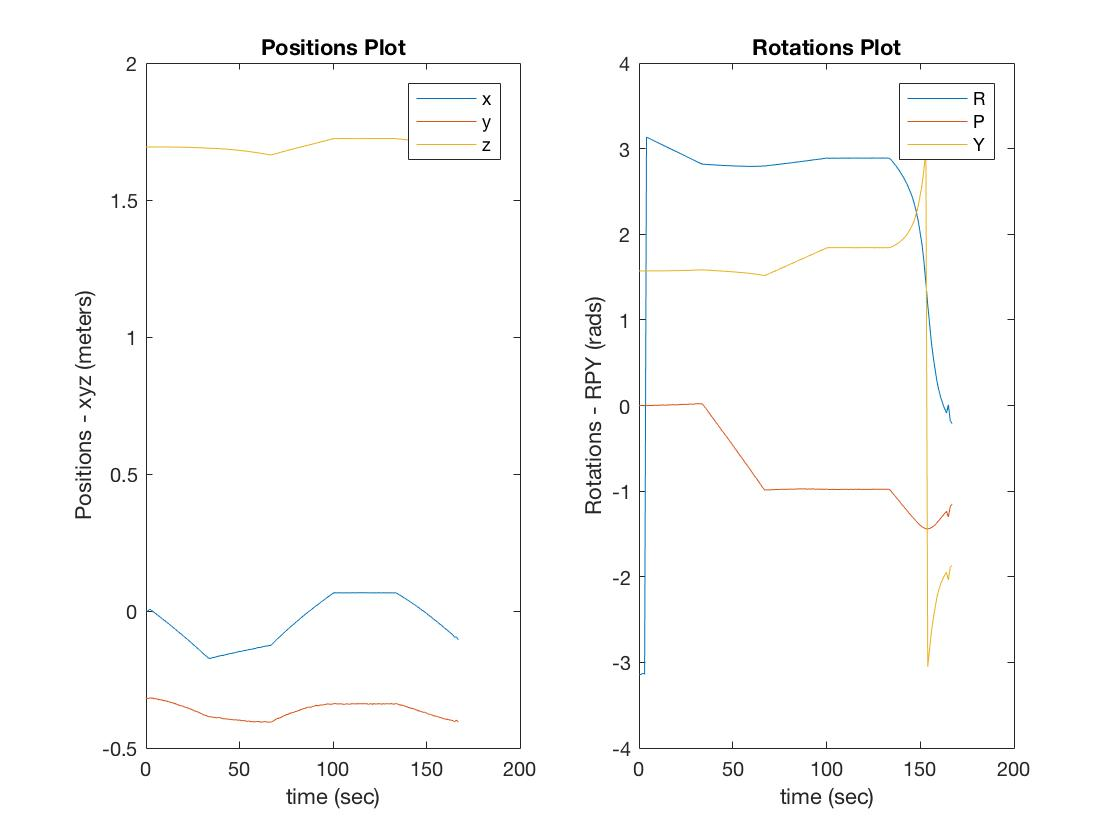
\includegraphics[width=0.49\linewidth]{fig/MediumSequence_tool_pose_M_Targ_Pts.jpg}
	}%
	\caption{Tool pose transformations}
	\label{fig:MediumSequenceToolPose}
\end{figure}

\subsubsection*{Fast Marker Sequence}
\begin{figure}[!htp]
	% Maximum length
	\subfloat[Tracking Single Point]
	{
		\label{fig:Fast1PointJoints}
		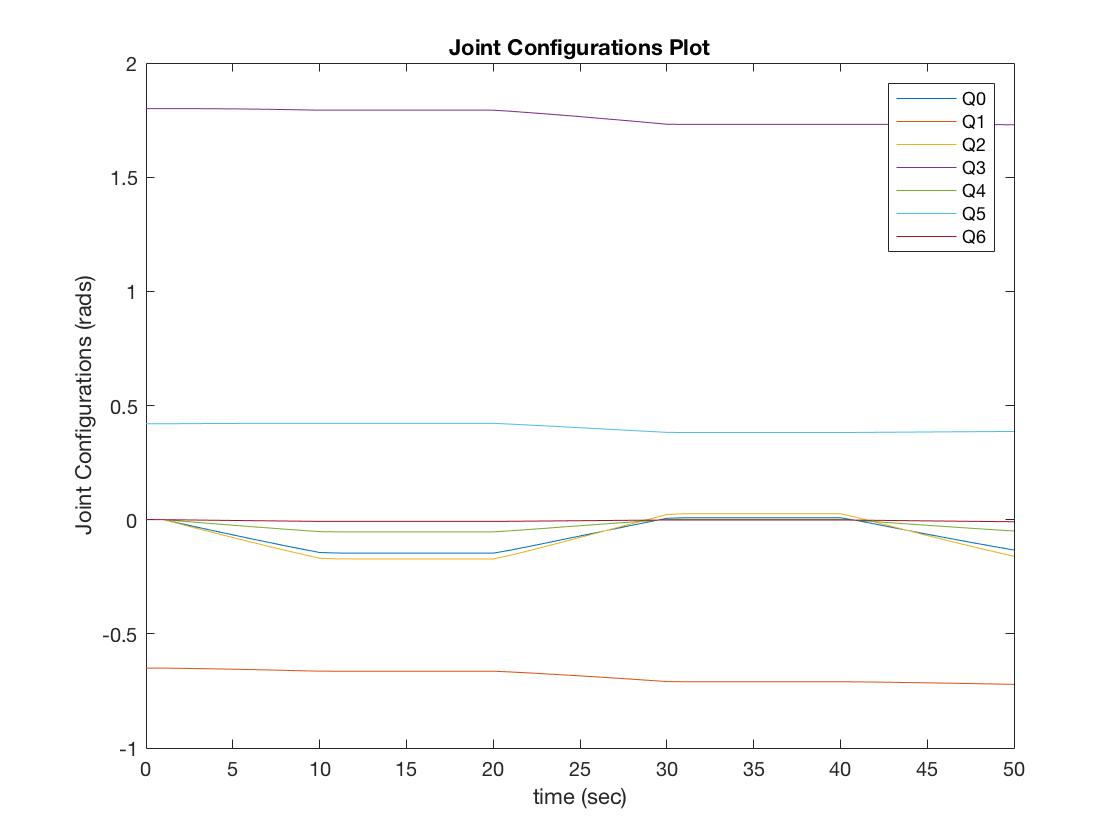
\includegraphics[width=0.49\linewidth]{fig/FastSequence_joints_1_Targ_Pt.jpg}
	}\hfill
	\subfloat[Tracking 3 Points]
	{
		\label{fig:Fast3PointsJoints}
		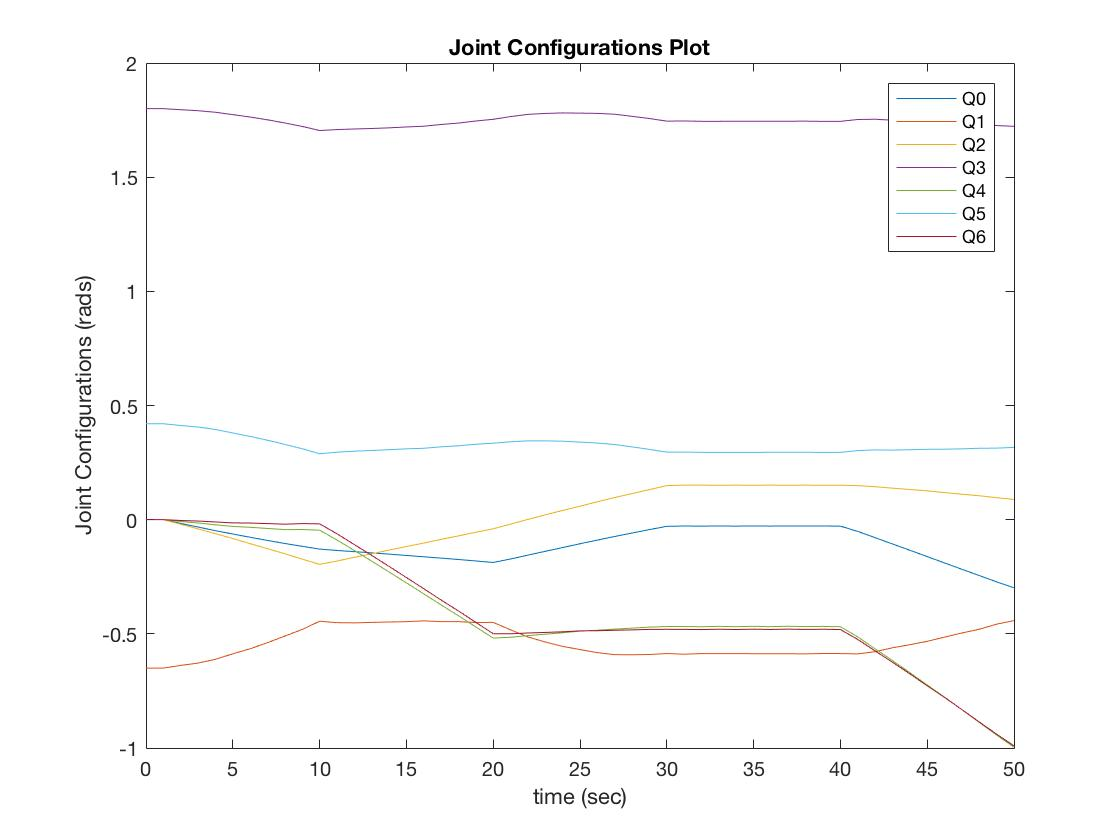
\includegraphics[width=0.49\linewidth]{fig/FastSequence_joints_M_Targ_Pts.jpg}
	}%
	\caption{Joint configurations}
	\label{fig:FastSequenceJoints}
\end{figure}

\begin{figure}[!htp]
	% Maximum length
	\subfloat[Tracking Single Point]
	{
		\label{fig:Fast1PointToolPose}
		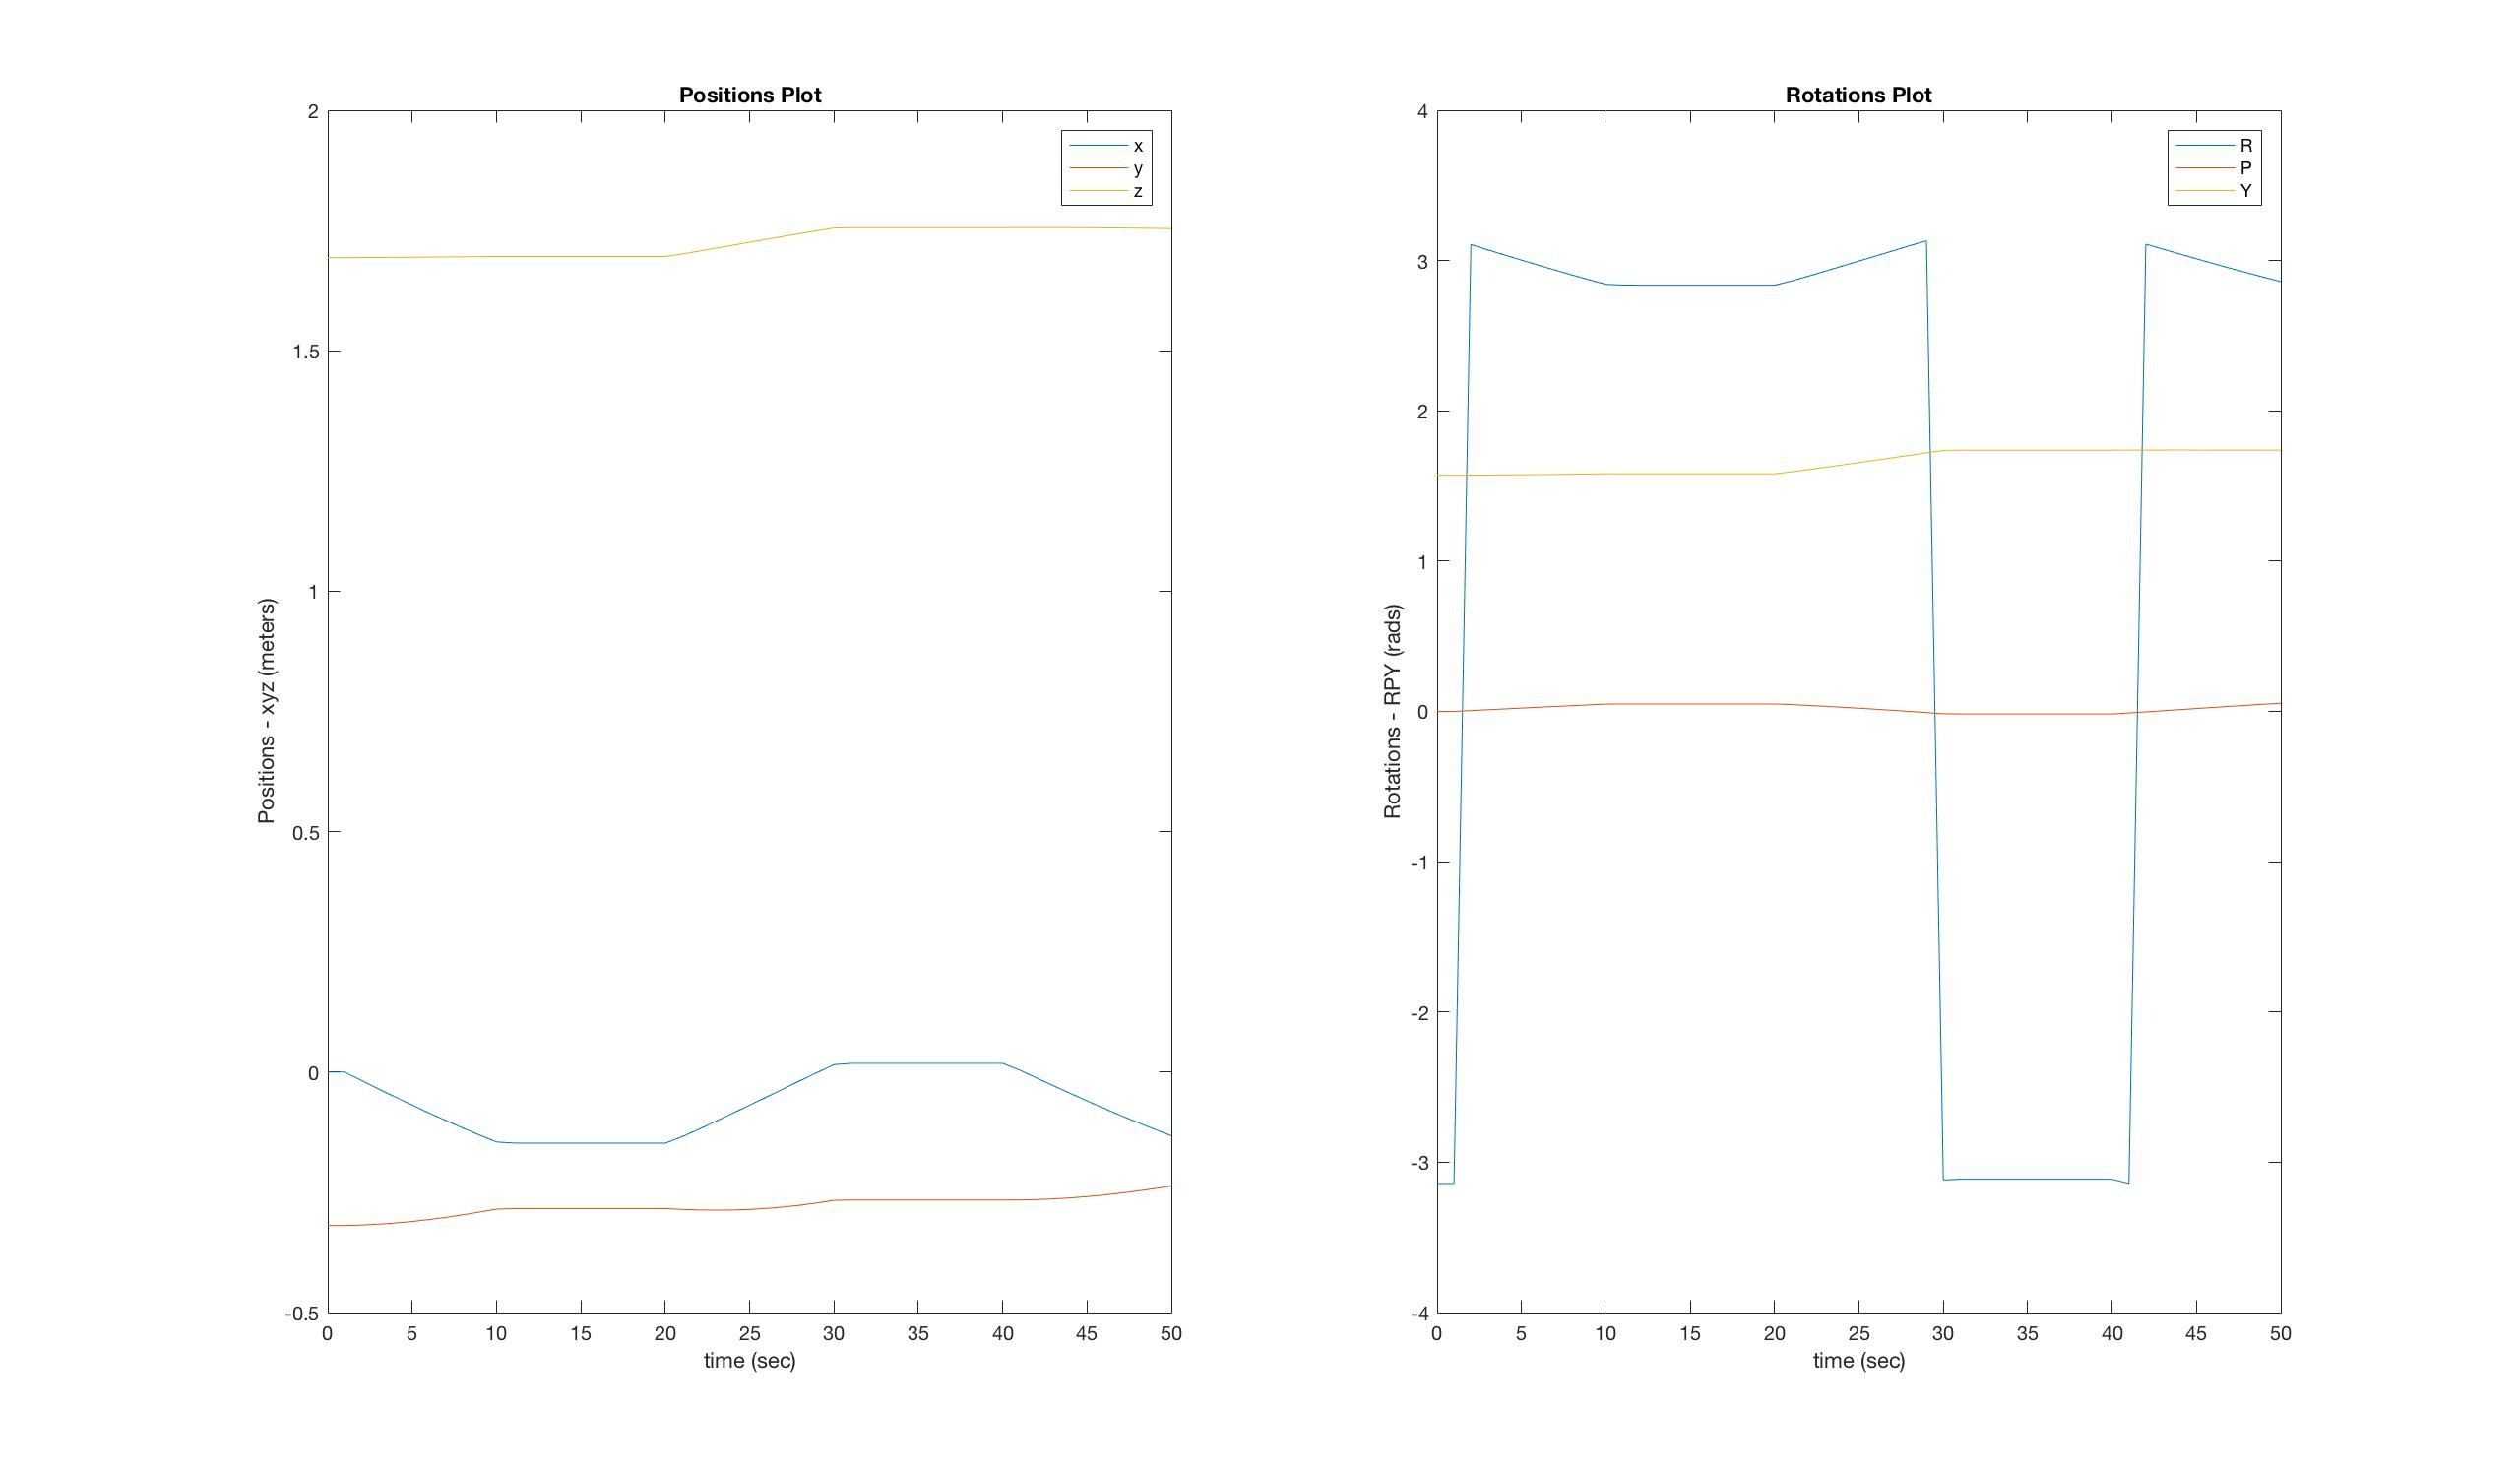
\includegraphics[width=0.49\linewidth]{fig/FastSequence_tool_pose_1_Targ_Pt.jpg}
	}\hfill
	\subfloat[Tracking 3 Points]
	{
		\label{fig:FastPointsToolPose}
		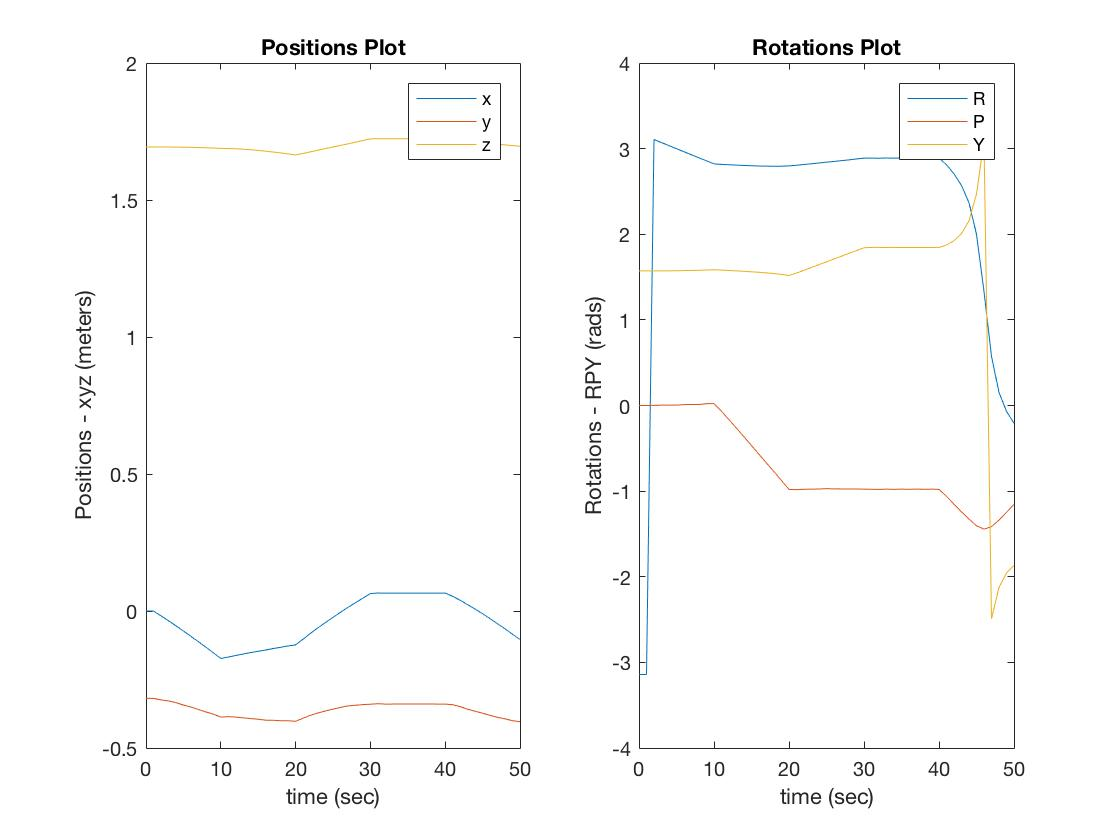
\includegraphics[width=0.49\linewidth]{fig/FastSequence_tool_pose_M_Targ_Pts.jpg}
	}%
	\caption{Tool pose transformations}
	\label{fig:FastSequenceToolPose}
\end{figure}
\end{document}
